\documentclass[a4paper]{article}

\usepackage[american]{babel}
\usepackage{amssymb}
\usepackage{array}
\usepackage{tabularx}
\usepackage{graphicx}

\usepackage{amsmath}
\usepackage{url}

\begin{document}

\title{{Folley: real-time fly noise origin locator} \\\large {Report of the 5LIU0 DBL project}}
\author{{Henk Oordt} \hfill
\\
{1717510} \hfill}

\begin{figure}
    \begin{center}
        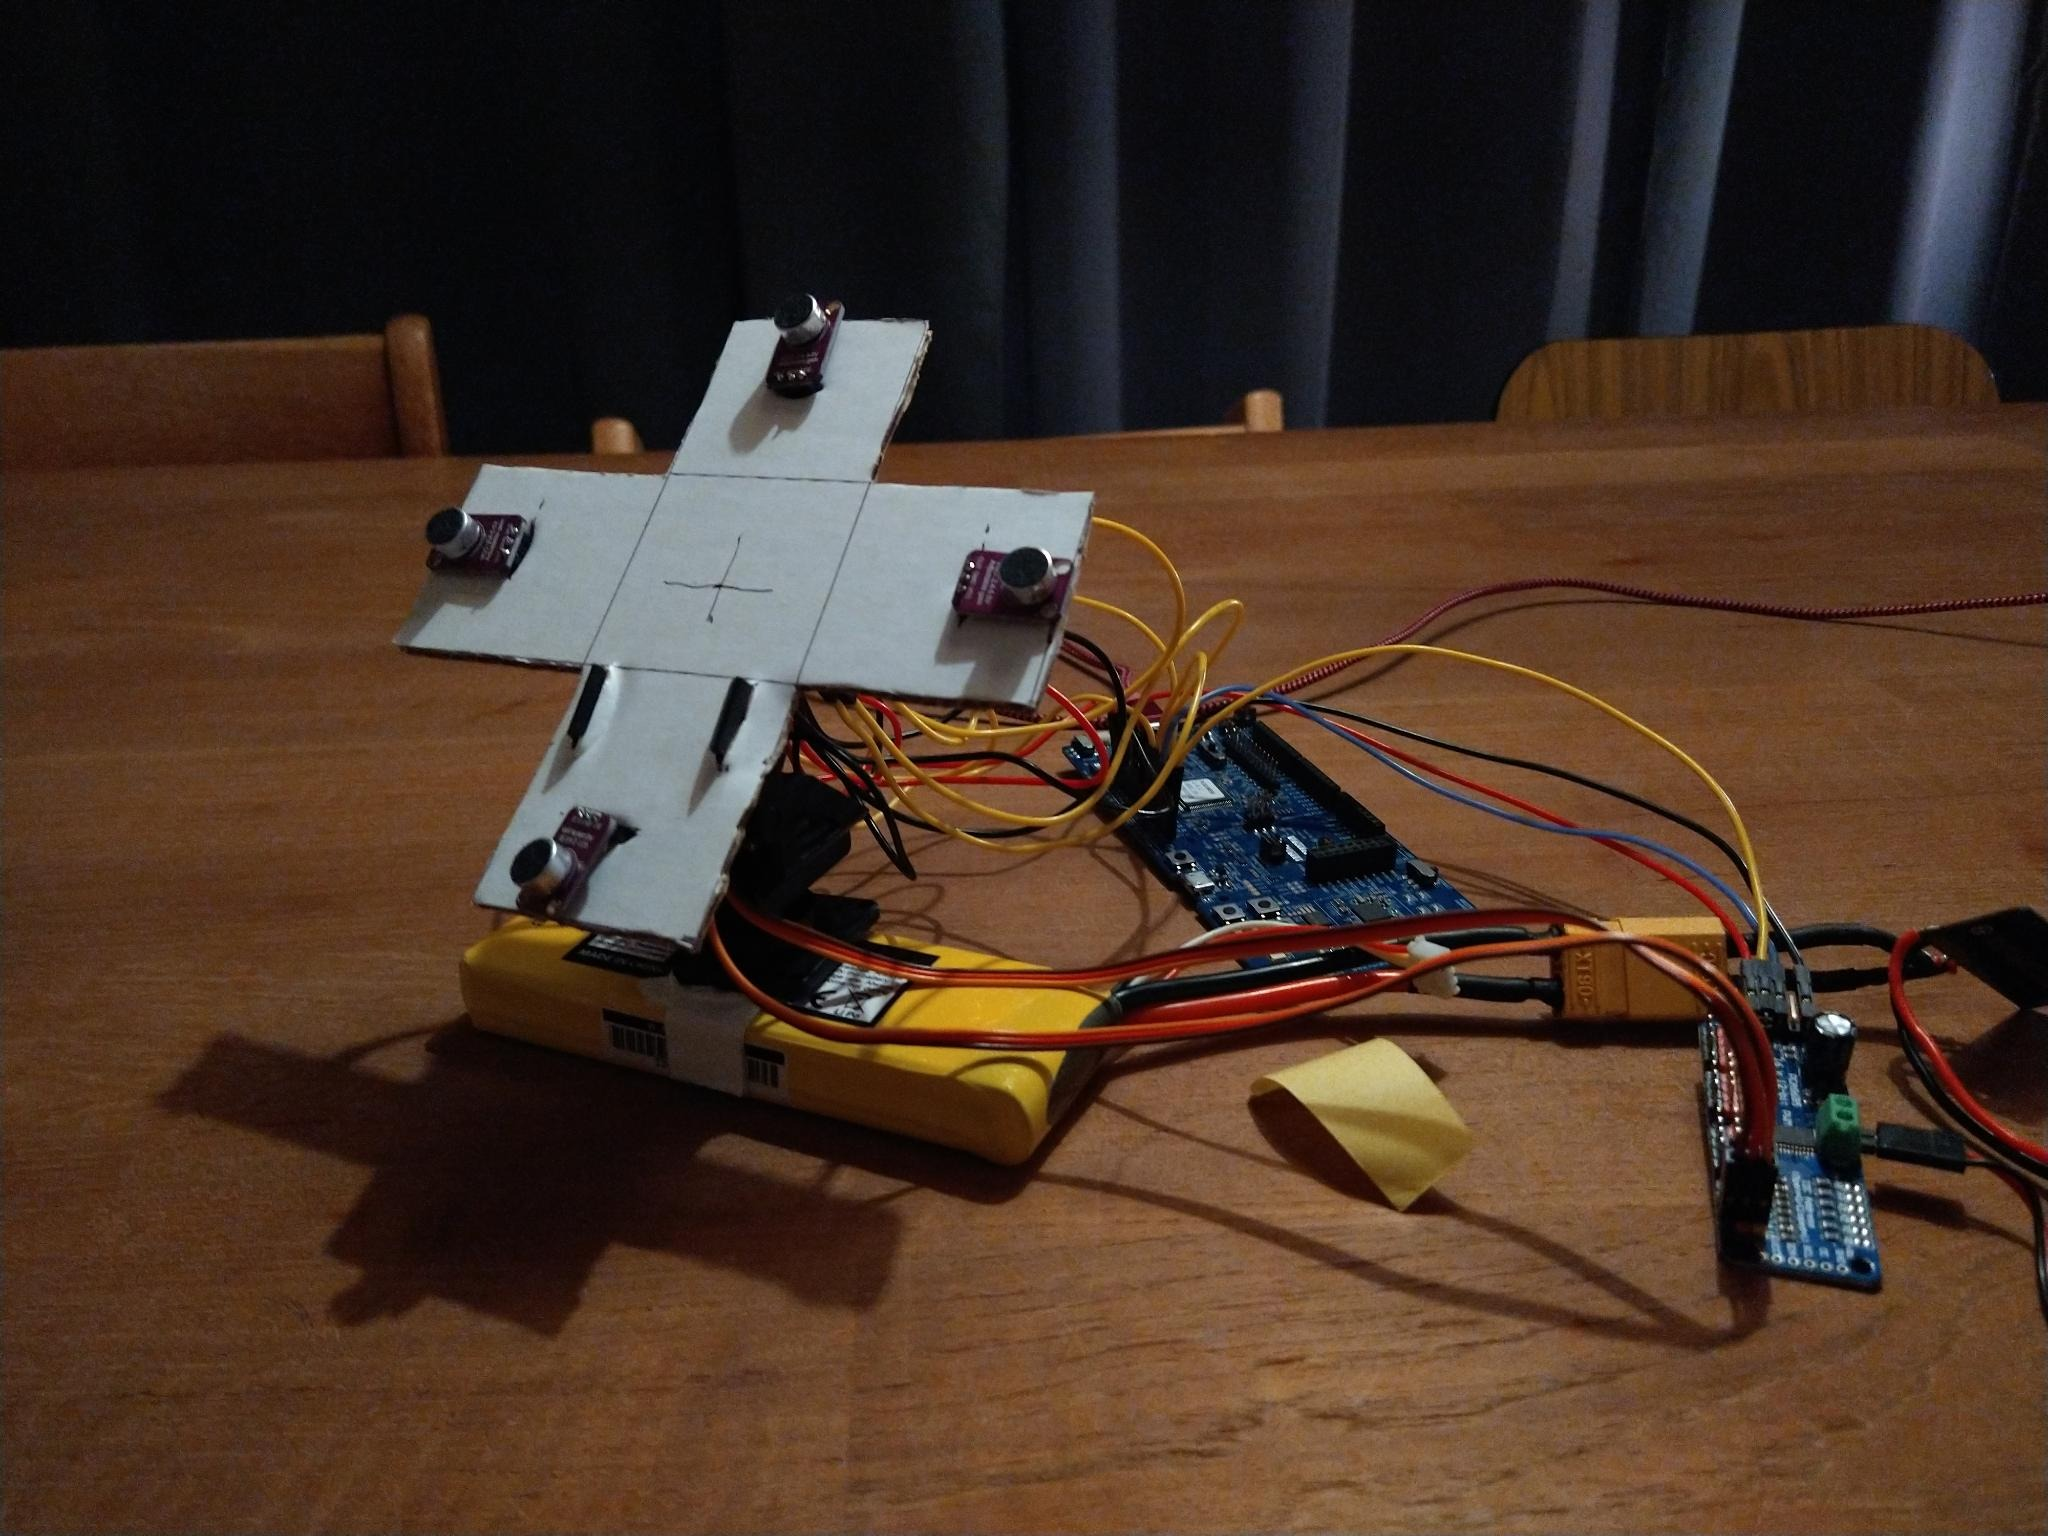
\includegraphics[width=\linewidth]{assets/device.jpeg}
    \end{center}
\end{figure}

\maketitle
\newpage

\section{Introduction}
% A general description of your project and its challenges.
Project `Folley' is aimed at the design and construction of a real-time sound origin locator. Folley uses audio signal analysis to detect and locate in 3D space the origin of the buzzing sound of flies. It then aims a low-power laser pointer in the direction of the origin of the sound.

In order to locate the sounds origin, Folley samples audio signal from an array of four analog microphones. The sampled signals are then analyzed in order to calculate a time-delay-angle-of-arrival (TDOA) \cite{6327613} which, along with the known microphone setup dimensions, can be used to calculate the azimuth and altitude angles of the origin with respect to the microphone array of the device.

In order to develop the TDOA analysis software, a set of Matlab \cite{matlab} scripts were written, which given the raw audio signal measurements, can calculate the azimuth and altitude angles of the sounds origin with respect to the microphone array. Essentially, in these scripts all of the signal analysis calculations that are needed to reach the project goals are implemented. These Matlab scripts will serve as a basis and a means of verification for the Rust implementation of the algorithm in firmware. Upon completion of the Matlab scripts and tweaking of parameters, the calculations have been re-implemented in Rust \cite{rust}, in order for the analysis to be done by the microcontroller on the nRF52840dk \cite{nrf52840-dk} board in real time. A simple command line application written in Rust that can communicate with the device and that converts raw microphone measurements to Matlab input files was developed as well.

This project focuses solely on the implementation of the TDOA analysis, as well as its evaluation. In this project, a testing environment was set up. This environment consists of a simple firmware application that is able to sample microphone data, and communicate these samples with the command line application that records them. The firmware is also able to control the pan-tilt bracket. The environment having been set up, a Matlab script has been implemented that is able to do the TDOA analysis based on four sine waves with separate phase differences, but with the same frequencies. Once this Matlab script had finished, the TDOA analysis was re-implemented in firmware, so that it can be done with microphone samples in real time. With the this project done, Folley should be able to locate origins of prefedined sine wave sounds, coming from a waveform generator.


\section{Problem specification}
% A detailed and technical description of the problem you’re addressing.
Flies and mosquitos emit a continuous buzzing sound in which certain frequencies and harmonics are present when flying around. This sound can be used to estimate the location of the insect. A device can use a set of microphones to analyze the sound signals as it is recorded by multiple microphones and obtain information about the location of the insect.

As the insect moves, the sound will come from different angles from the device perspective. For both the x and y axis, the time of arrival of the buzzing sound can be used to calculate the angle from which it originated. In figure \ref{fig:problem_overview}, a schematic overview of the problem is given for a single axis. A sound source produces a sound. The origin is assumed to be infinitely far away, so the sound is moving in straight waves when it arrives at the microphone array. In this example, the sound hits microphone 2 before it hits microphone 1. Let $d$ be the distance travelled by the sound between the moment it hits microphone 2 and the moment it hits microphone 1 and $d_{mics}$ be the distance between the microphones. Then, a right triagle can be formed with a hypotenuse of length $d_{mics}$, one side of length $d$ and an angle $\theta$ between them. In order for $\theta$ to be calculated, the following equation is used:\[\theta = \arctan(\frac{d}{d_{mics}})\] $\theta$ equals the angle between the device and the sound origin. $\theta$ ranges from $0^{\circ}$ to $90^{\circ}$ to $180^{\circ}$ as the source is moved from the right, to the middle, towards the left of the array. 

Given the delay $t_{delay}$ in time between the moment the sound hits microphone 1 ($t_1$) and the it hits moment microphone 2 ($t_2$), with $t_{delay} = t_1 - t_2$ $d$ can be derived as follows:\[d = t_{delay} \cdot V_{sound}\]where $V_{sound}$ is the speed of sound, $343\ m/s$

The challenge for this project is to find $t_{delay}$ given just the raw microphone samples from ADC of the microcontroller. Also, a suitable value for $d_mics$ needs to be found in order for the device to be able to work with typical mosquito buzzing sound, keeping in mind its periodicity.

\begin{figure}
    \begin{center}
        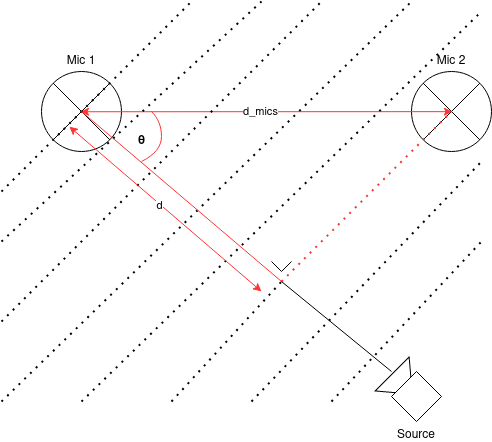
\includegraphics[width=25em]{assets/problem_overview.png}
        \caption{Problem overview}
        \label{fig:problem_overview}
    \end{center}
\end{figure}

To estimate $t_{delay}$, we can use cross-correlation of two signals. Using cross-correlation, the precense of one signal can be detected within another signal. It is a measure of similarity between two signals as one signal is delayed with respect to the other. For discrete signals, cross correlation between real-value signals $x$ and $y$ is defined as follows: \[(x \star y)[n] \triangleq \sum_{m = -\infty}^ {\infty} x[m]\cdot y[m + n]\] This yields a new signal, of which the $n$ corresponding the highest value is the delay between the signals for which they were most similar. Therefore, the delay between the signals $x$ and $y$ in terms of number of samples, $n_{delay}$ can be found with \[n_{delay} = \underset{n}{\mathrm{argmax}}\ (x \star y)[n]\] Given a fixed sample period $T_s$ used for both signals, $t_{delay}$ can be calculated with \[t_{delay} = n_{delay} \cdot T_s\]

$t_{delay}$ has a maximum at $\theta = 180^{\circ}$ and a (negative) minimum at $\theta = 0^{\circ}$. Therefore, the calculations can be optimized by only calculating the cross correlation for a limited range of $n$. The upper limit of $n$, $n_{max}$, can be found by \[n_{max} = \frac{d_{mics}}{T_s \cdot V_{sound}}\] The minimum is found by $n_{min} = -n_{max}$. Given these limits, the length of the cross correlation signal can be reduced drastically:\[(x \star y)[n] \triangleq \sum_{m = n_{min}}^ {n_{max}} x[m]\cdot y[m + n]\] If the wave length $\lambda$ is no bigger than $d_{mics}$, using the limited cross correlation also makes the cross correlation suitable for periodic sigals: the signals will only optimally lined up for one value of $n$.

This completes the set of calculations needed to calculate $\theta$ given two signals. In this project, before calculations were implemented in order to find a suitable value for $d_{mics}$, and for the analysis to be done on-device in real time.

\section{Evaluation criteria}
% How will you be able to determine if your project is successful? Try to find objective and quantitative metrics.
In order to indicate whether the project a success, the following goal is defined. The TDOA analysis is able to calculate the azimuth and altitude angles within a 10 degree error margin 80\% of the time, when presented with a predefined sine wave sound.

As the accuracy of the pan-tilt servos is low, the accuracy of the actual laser pointer is not measured. Only the calculation outputs are benchmarked, both the Matlab script and the firmware implementation.

\section{Setup}
% What are the signals (real, simulated or physical) that you will use for your project? What is the hardware and/or software setup that you have used?

The device uses an array of four electret microphones, mounted in a `+'-shape. As can be seen in figure \ref{fig:mic_array_dimensions}, every two opposite microphones are 125mm apart. Using this setup, it becomes possible to esimate the angle from which the buzzing sound comes from in both the horizontal and vertical axis. 

\begin{figure}
    \begin{center}
        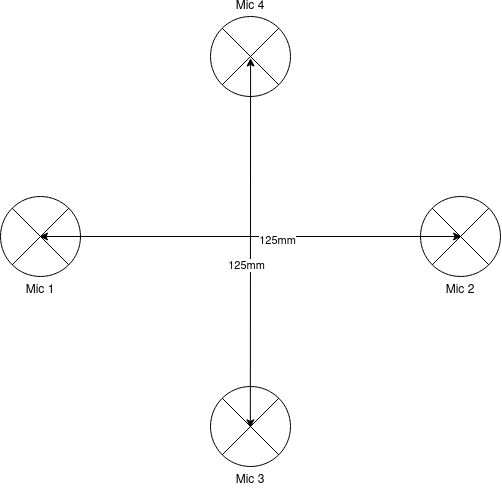
\includegraphics[width=25em]{assets/mic_array_dimensions.png}
        \caption{Microphone array dimensions}
        \label{fig:mic_array_dimensions}
    \end{center}
\end{figure}


\begin{enumerate}
    \item Microphone array set up
    \item Signals are analog microphone output voltages, amplified by on-board opamp
    \item Sampled and quantized by nRF52840 on-chip ADC, into 12-bit 2's complement numbers
\end{enumerate}

\begin{figure}
    \begin{center}
        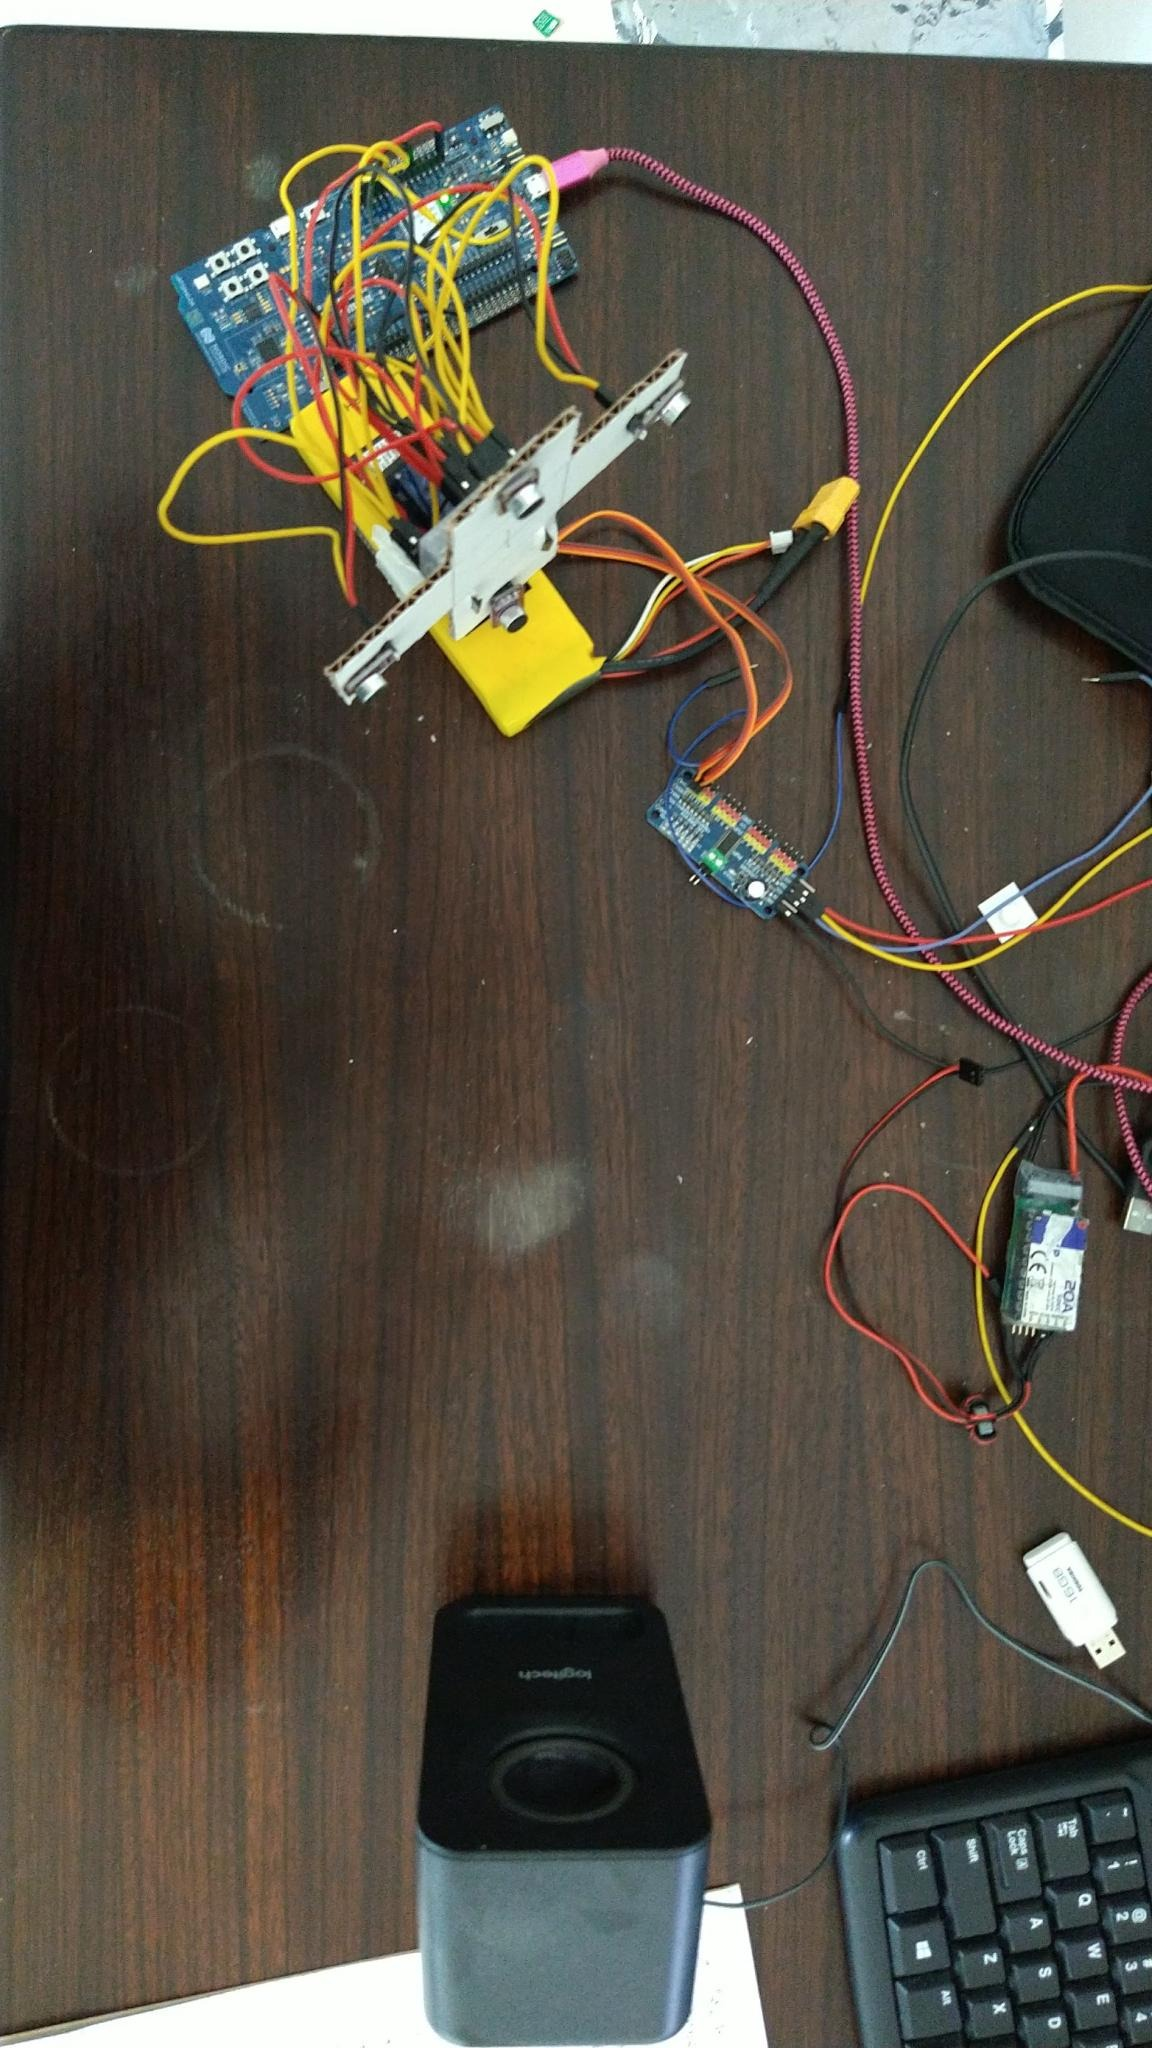
\includegraphics[angle=90,width=\linewidth]{assets/test_setup.jpeg}
        \caption{Setup for measuring}
        \label{fig:test_setup}
    \end{center}
\end{figure}


The microphone array as well as the laser diode is mounted to a servo-powered pan-tilt bracket, which is being used to point the microphones and the laser diode in the direction of the origin of the sound given the TDOA analysis output. All of this is controlled by a Nordic Semiconductor nRF52840 microcontroller, mounted on a nRF52840DK board, for which firmware is to be customly written in Rust \cite{rust}. This microcontroller is able to sample up to 8 analog inputs, and can control the servo motors of the pan-tilt bracket using pulse-width modulation (PWM) \cite{GULYAEV20161529} with the help of a PCA9685 \cite{pca9685} PWM controller, significantly simplifying the control of the pan-tilt bracket positioning. The nRF52840dk board can also relatively easily be set up for serial communication over USB \cite{usb}, enabling running real-time analysis and graph plotting on a host computer for development ease.


\section{Approach}
% A detailed, technical description how you solved the problem.

\begin{enumerate}
    \item Signal is periodic, therefore take into account that the delay is always less than 1 period. Output of cross-correlation is the number of samples the reference leads or lags the other microphones signal.
    \item Given sample rate, the distance between microphones and the speed of sound, the delay is used to calculate the angle from which the sound came. The distance between the device and the sound origin, is assumed to be infinitely large so the sound waves are assumed to be straight once hitting the microphones.
    \item Output of calculation is used to point the laser into the direction of the sound.
\end{enumerate}

\section{Results and Analysis}
% Evaluation of the results using the defined criteria and a reflection on the outcomes, explanations for shortcomings, ideas for improvements.
\begin{enumerate}

    \item Sound used in analysis played from smartphone at various angles multiple times. Measurements recorded, fed into matlab scripts and CLI. Output and error noted
    \item Same sound played from smartphone, as real-time analysis by device outputs the angles.
    \item graphs
\end{enumerate}


% baseline
\begin{table}
    \begin{center}
        \begin{tabular}{ | m{5em} | m{2em} | m{3.5em} | }
            \hline
            File name    & N   & Average ($^{\circ}$) \\
            \hline
            \hline
            baseline.txt & 101 & 90                   \\
            \hline
        \end{tabular}
        \caption{\label{tab:results_baseline}Results from testing with 1100Hz sine wave signal.}
    \end{center}
\end{table}

% sine_1100hz
\begin{table}
    \begin{center}
        \begin{tabular}{ | m{5em} | m{4em}| m{2em} | m{3.5em} | m{3.5em} | m{3.5em} | m{3.5em} | m{2.5em} | }
            \hline
            File name                  & Expected angle ($^{\circ}$) & N   & Average ($^{\circ}$) & Standard deviation & Passed samples & Pass percentage & Test passed \\
            \hline
            \hline
            0\textunderscore deg.txt   & 0                           & 101 & 24                   & 0                  & 0              & 0               & false       \\
            \hline
            45\textunderscore deg.txt  & 45                          & 101 & 53                   & 0                  & 101            & 100             & true        \\
            \hline
            90\textunderscore deg.txt  & 90                          & 101 & 90                   & 0                  & 101            & 100             & true        \\
            \hline
            135\textunderscore deg.txt & 135                         & 101 & 114.42               & 1.66               & 0              & 0               & false       \\
            \hline
            180\textunderscore deg.txt & 180                         & 101 & 156                  & 0                  & 0              & 0               & false       \\
            \hline
        \end{tabular}
        \caption{\label{tab:results_sine1100hz}Results from testing with 1100Hz sine wave signal.}
    \end{center}
\end{table}

% mosquito
\begin{table}
    \begin{center}
        \begin{tabular}{ | m{5em} | m{4em}| m{2em} | m{3.5em} | m{3.5em} | m{3.5em} | m{3.5em} | m{2.5em} | }
            \hline
            File name                  & Expected angle ($^{\circ}$) & N   & Average ($^{\circ}$) & Standard deviation & Passed samples & Pass percentage & Test passed \\
            \hline
            \hline
            0\textunderscore deg.txt   & 0                           & 101 & 32.07                & 20.21              & 0              & 0               & false       \\
            \hline
            45\textunderscore deg.txt  & 45                          & 101 & 56.29                & 8.24               & 75             & 74              & false       \\
            \hline
            90\textunderscore deg.txt  & 90                          & 101 & 90                   & 0                  & 101            & 100             & true        \\
            \hline
            135\textunderscore deg.txt & 135                         & 101 & 128.72               & 11.03              & 91             & 90              & true        \\
            \hline
            180\textunderscore deg.txt & 180                         & 101 & 146                  & 22.81              & 0              & 0               & false       \\
            \hline
        \end{tabular}
        \caption{\label{tab:results_mosquito}Results from testing with mosquito sound.}
    \end{center}
\end{table}




\section{Conclusions}
% (Short) What did you learn from doing the project? What solutions did you provide?


\bibliographystyle{plain}
\bibliography{references}
\end{document}
